\documentclass[11pt,twoside,a4paper]{article}
%--------------document formatting-------------%
%---------------The necessary Packages------------%
\usepackage[backend=biber]{biblatex}
\usepackage{graphicx}
\usepackage[]{siunitx}
\usepackage{textcomp}
\usepackage{gensymb}
%---------------metadata--------------------%
\author{Abhishek Anil Deshmukh\\
	and
	Sweta Singh\\}
\title{Summer Internship Report}

%-----------------Starting--------------------%
\begin{document}

\maketitle

\section{Heat Shock}
Heat Shock  is given to cells for getting the mutant plasmids into them, We keep them in a temperature of -4 \textdegree C for 15 minutes then move them to 42 \textdegree C for 35 seconds and the move back to -4\textdegree C.

In this process all the plasmids do not enter the cells, so you incorporate a X-Resistant gene into the plasmid (Here X can be anything, we chose Amphicilin) and now after incubation of about an hour in a rich medium at 220RPM and 37 \textdegree C. After that colony making is done at 37 \textdegree C for atleast 12 hrs (we did it for about 18 hrs).

\section{Ultracompetent Bacterial Cells}
These are the cells which clone plasmids for large number of them.(Basically PCR for large sequences)

PCR has a limit of about 4kb, so for cloning large sequences Ultracompetent Bacterial Cells are used.

These cells are given a heat shock and them left in medium for an hour, later on they are taken for colony making for atleast 12 hrs at 37 \textdegree C.
\section{lb Broth Preparation}
2.5gm of lb broth powder per 100 ml of water, the boxes of lb broth and lb agar look surprisingly similar, so watch out for that. 4mg of lb agar powder per 100ml of water. If we are making x ml of lb broth solution then the size of the container should be 5x to 6x ml as the size increases when bacterial or cells feed on it.

\section{Competence}
The ability of a cell to alter its own genetics by taking up extracellular DNA from the environment. It is brogth into cell by environmental conditions like starvation. Condotions inducing sporation often over lap with condition inducing competence.

\section{Transformation}
It is a process in which the competent cell intakes DNA from outside and ends up changing its own DNA transformation usually produces a mixture of relatively few transformed cells and an abundance of non-transformed cells, a method is necessary to select for the cells that have acquired the plasmid.
The plasmid therefore requires a selectable marker such that those cells without the plasmid may be killed or have their growth arrested. Antibiotic resistance is the most commonly used marker for prokaryotes. .
\section{Conjugation}
At the 8\textsuperscript{th} hour
\begin{figure}
	\centering
	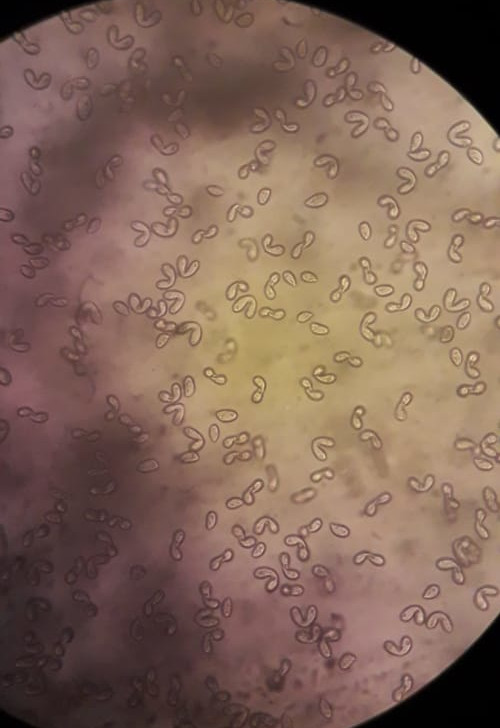
\includegraphics[width=0.6\textwidth]{images/conjugation1.jpeg}
	\caption{Conjugation}
	\label{conjugation1}
\end{figure}

\section{Agarose-Gel}
For 100ml of agarose gelcast of 0.8%, it takes 0.8g of agar and 100ml fo 1x TAE( It's a buffer)
\begin{enumerate}
	\item Tape the gel caste tray
	\item Put the comb on the end of the cast tray
	\item Agar(0.8g)+ 1x TAE(100mL) in a flask
	\item Oven it till dissolution (In this case it took about 5 minutes), check after every minute or so.
	\item Let the flask cool before putting in ETB, but don't let it cool so much as to start polymerization.
	\item Put in EtBr(2\textmu{}L) shake well.
	\item Put it in the tray
	\item Move the bubbles away from the well, towards the ends.
\end{enumerate}

\section{Cell Fixation}
Cell fixation is the process of arresting the cells completely till the protein level. This can be done in two ways.
\begin{enumerate}
	\item PFA

		Paraformaldehyde. The sample of cells are centrifuged to precepetate, the floating part is thrown away, PFA is added quickly. After sometime the cells are suspended again, to the original concentration.
	\item Cooling

		This process involves slow cooling down of the cells.
\end{enumerate}

\section{Cell Counting}
Hemocytometer is a counting-chamber device orginally designed and usually used for counting blood cells.
\begin{enumerate}
	\item Take a batch of starved cells(basically anycells which you want to find the cell count).
	\item Fix them with PFA(0.5\textmu{}L)
	\item Add the solution(10\textmu{}L/ chamber) in both the chambers.(keep the pippet horizontal for faster spreading)
	\item Allow the chanber to fill(Thanks to capillary action, interference is not required).
	\item View under the microscope.
	\item Determine the no.of cells

		Count the number of cells in each square, 4 squares in each chamber,count both the chambers.
		Divide the number by 80.(divide by 8 so we get average number per square and them by 10 because of the constant)
		The number which we get is that many million cells/mL.
\end{enumerate}

\section{DAPI Staining}
 4,6-diamidino-2-phenylindole(DAPI) staining is the process of arresting the cells and staining them with a UV Sensitive dye(DAPI).
\begin{enumerate}
	\item Centrifuge 1ml of cell under 1.1G for 2 minutes and discard the supernatant(the floating stuff).
	\item PFA 500\textmu{}L(At the time when you want to arrest them)(In our case at 8 hours for when they were kept together).
	\item Tap and Invert.
	\item Centrifuge under 1.1G for 2 minutes and discard the supernatant(the floating stuff).
	\item Add 200\textmu{}L of 10mM Hepes(A buffer), tap and Invert.
	\item Centrifuge under 1.1G for 2 minutes and discard the supernatant(the floating stuff).
	\item Add 200\textmu{}L of DAPI.(Preferabely in dark)
	\item Leave in dark for 10 minutes.
	\item Centrifuge under 1.1G for 2 minutes and discard the supernatant(the floating stuff).
	\item Take 5\textmu{}l of cells and prepare slide.
\end{enumerate}
DAPI is light sensitive so stored in darkness in fridge.

\section{DMC Preparation}
Be very precautious of contamination while making it.
\begin{enumerate}
	\item Use autoclaved MQ
	\item discard old DMC from the DMC deducted bottle.(each and every drop)
	\item Preparation Requirements
		\begin{enumerate}
			\item \[ Na_2 HPO_4 \]
			\item \[ NaH_2PO_4\]
			\item Sodium Citrate
			\item \[ CaCl_2 \]
			\item MQ water
			\item renin pipette (1ml)
		\end{enumerate}
\end{enumerate}
Procedure for Preparation:-
\begin{enumerate}
	\item Add 1ml of \[ NaH_2PO_4 \]. Then 1ml \[ Na_2HPO_4 \]
	\item Add 100mm Sodium Citrate (1.7ml).
	\item Add 100mm Calcium Chloride (1.5ml).
	\item In measuring cylinder pour exactly 1L autoclaved MQ.
	\item Remove 5.2mL of Autoclaved MQ by renin pipette and pour in DMC bottle.
	\item Place cap and mix properly.
	\item Autoclave it for 40 mins along with \[ CaCl_2 \] and \[ MgCl_2 \].
	\item After 12-14 Hrs it is ready for starvation.
\end{enumerate}

\section{Western Blotting}
\begin{enumerate}
	\item Blotting Buffer(50ml) :- 10ml Methanol +  35ml Water + 5ml 10 x WesternBlot Buffer
	\item 6 cm x 8 cm Blotting paper/PVDF Membrane/NitroCellullose Membrane
	\item 6 Blotting Sheets
\end{enumerate}
Do not touch the membrane.

Set the semi-dry unit to 17V for 45 Min and 2.5A as the limit.
\begin{enumerate}
	\item Dip the PVDF membrane in methanol(for 5 to 10 mins to activate it).
	\item Throw away the methanol.
	\item Add the complete(50ml) Blotting Buffer in the same container and put in the 6 blotting sheets to soak for about 6 minutes.
	\item Wet the base of semi-dry unit with buffer.
	\item Put in 3 sheets.
	\item Then put the membrane on it with a forcep.(make sure to remove the air bubbles)
	\item Cutoff the unwanted parts of the gel-cast
	\item Now put hte gel-cast with protien on it.
	\item Put the other 3 sheets onto the gel-cast.(again make sure to remove the air bubbles)
	\item turn on the semi-dry unit and leave it for 45 minutes.

		While the protien is going from gel to the membrane make the Blocking solution.

		Blocking Buffer(100ml):- 10ml 10xTBS + 90ml MQ + 3gm SM Powder + 100\textmu{}l Tween-20
	\item When done with 45 minutes take the membrane out and keep with Blocking solution(100ml) for 1 hr on rocking table.
	\item Throw away the Blocking solution
	\item Put in the Primary antibody and soak for 60 minutes.
	\item Throw away Primary antibody and wash with Blocking Buffer thrice for 10 minutes each.
	\item Put in the Secondary antibody and soak for 90 minutes.
	\item Throw away Secondary antibody and wash with Blocking Buffer thrice for 10 minutes each.
	\item Develop with ECL.
	\item Image in Chemidock.
\end{enumerate}

\section{Protien Purification}
The following measurements are for 500ml of cells use by your descretion.
\begin{enumerate}
	\item Centrifuge at 4 \textdegree C at 12k RPM for 5 mins and throw away the superlatent.
	\item Add Protiase Inhibitor(200\textmu{}l).

		So that after the cell covers are broken the protiases are not binded to the protine to be purified.
	\item 1mg/ml lysozime (To break the cell wall)
	\item Add 40ml of Buffer for resuspension then mix using pippet till pellet is dissolved.
	\item Incubate in cold room for 40 mins.
	\item Sonicate for 5 minutes at 60\% amplitude with 3sec on and 3sec off pulsation.
\end{enumerate}
\end{document}
